% !TEX program = xelatex
\documentclass[10pt,twocolumn,a4paper]{article}
\usepackage{fontspec}
\setmainfont{Times New Roman}
\usepackage[vietnamese]{babel}
\usepackage[top=20mm,bottom=20mm,left=15mm,right=15mm]{geometry}
\usepackage{amsmath, amsfonts, amssymb}
\usepackage{graphicx}
\usepackage{booktabs}
\usepackage{array}
\usepackage{cite}
\usepackage{caption}
\captionsetup{font=small,labelfont=bf,justification=centering}
\usepackage[hidelinks]{hyperref}

\title{\textbf{Gọi Công Cụ (Tool Calling) Tiếng Việt: Nghiên Cứu So Sánh Giữa Mô Hình Ngôn Ngữ Nhỏ End-to-End Và Kiến Trúc Chuyên Biệt Bi-Encoder + Cross-Encoder}}

\author{
    \textbf{Đào Phước Thịnh}$^{1}$, \textbf{Hà Quang Đạt}$^{1}$, \textbf{Đặng Văn Thìn}$^{1,*}$ \\[0.2cm]
    $^{1}$Khoa Công nghệ Thông tin, Trường Đại học Công nghệ Thông tin, ĐHQG-HCM, Việt Nam \\
    Email: \texttt{\{21521469, 21521925\}@ms.uit.edu.vn}, \texttt{thindv@uit.edu.vn} \\
    $^{*}$Tác giả liên hệ
}

\date{Năm 2026}

\begin{document}

\maketitle

\begin{abstract}
\textbf{Tóm tắt}---Gọi công cụ (tool calling) là cơ chế then chốt giúp tác tử AI tương tác với các API bên ngoài, song việc ứng dụng trên tiếng Việt gặp rào cản về độ trễ tự hồi quy cao, nguy cơ lỗi cú pháp JSON và bùng nổ bộ nhớ ngữ cảnh. Bài báo này thực hiện so sánh đối đầu thực nghiệm giữa Mô hình Ngôn ngữ Nhỏ End-to-End (SLM Qwen3.5 2B/4B) và Hệ thống phân tách không tự hồi quy (Bi-Encoder BGE-M3 kết hợp Hierarchical Cross-Encoder XLM-RoBERTa) trên hai benchmark: Canonical Core (77,028 cặp song ngữ) và CustomTools-VI (8,000 mẫu bản địa). Kết quả cho thấy SLM 4B sau hiệu chuẩn âm tính đạt ArgA 87.92\% (seen) và 86.75\% (unseen), Non-FC Recall 100.0\% và cao hơn GPT-5.6 Luna trên giao thức CustomTools-VI. Trong stress test, Method 2 ghi nhận P50 55.13–107.68 ms, PyTorch allocated VRAM khoảng 3.21 GiB và lỗi cú pháp 0\% theo định nghĩa structured-output; các số đo được thu thập theo protocol riêng. Khi mở rộng tới 1,000 công cụ, Method 2 duy trì ArgA 84.00\%, trong khi SLM gặp CUDA OOM tại $N \ge 500$ trên GPU 16GB. Nghiên cứu cung cấp cơ sở định lượng cho việc lựa chọn kiến trúc theo yêu cầu chất lượng và tài nguyên.

\textbf{Từ khóa:} Gọi công cụ, mô hình ngôn ngữ nhỏ, Bi-Encoder, Cross-Encoder, trích xuất tham số, tiếng Việt.
\end{abstract}

\vspace{0.3cm}
\textbf{\textit{Từ khóa}}---Gọi công cụ (Tool Calling), Mô hình ngôn ngữ nhỏ (SLM), Bi-Encoder, Cross-Encoder, Trích xuất tham số, Kiểm thử áp lực, Tác tử AI tiếng Việt.

\vspace{0.5cm}

\section{Giới Thiệu (Introduction)}

Khả năng gọi công cụ (tool calling), thường được gọi là gọi hàm (function calling), là cơ chế nền tảng giúp các mô hình ngôn ngữ lớn (LLM) và các tác tử thông minh (AI Agents) kết nối với thế giới bên ngoài. Thông qua việc phân tích ngôn ngữ tự nhiên của người dùng và định nghĩa schema của các công cụ khả dụng, mô hình tự động nhận diện thời điểm cần kích hoạt công cụ, lựa chọn chính xác API mục tiêu và trích xuất các tham số cấu trúc tương ứng.

\begin{figure}[htbp]
    \centering
    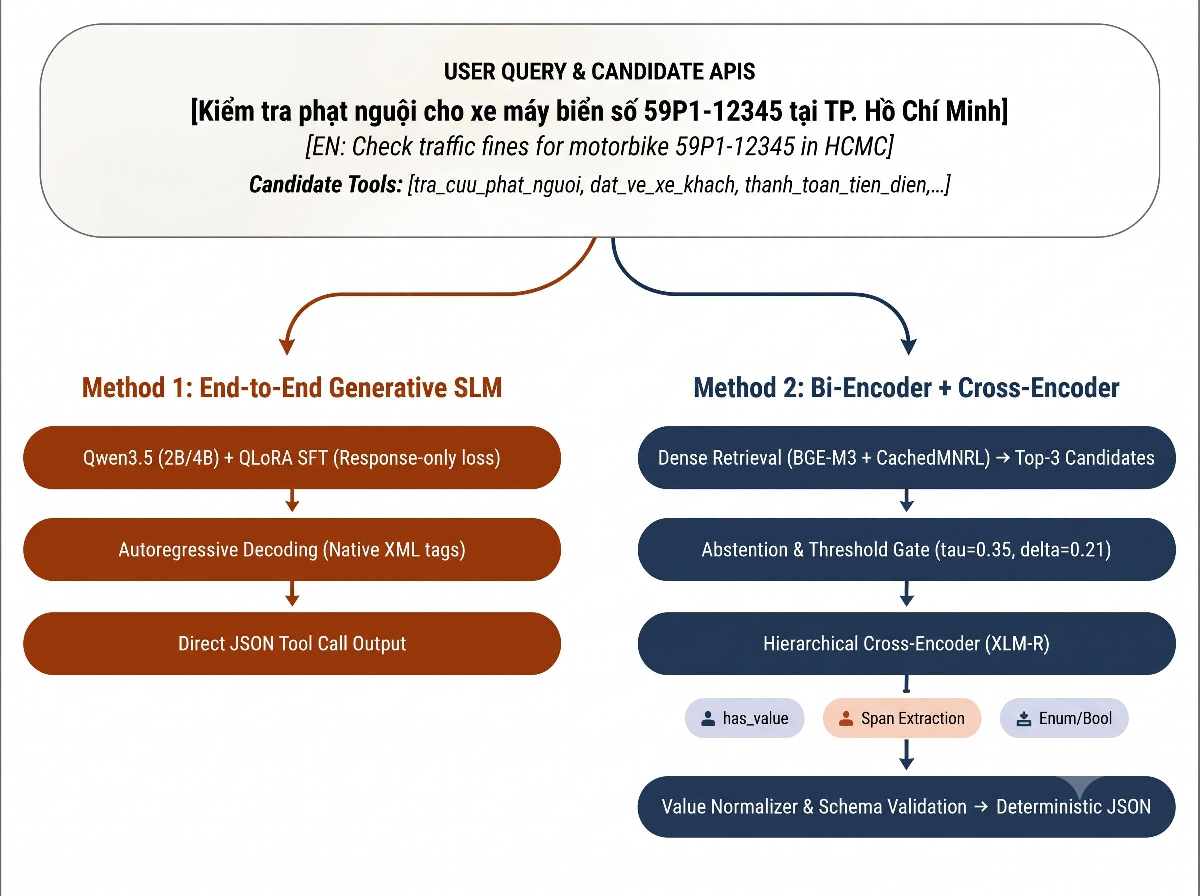
\includegraphics[width=0.88\textwidth]{figures/fig1_system_architecture}
    \caption{Sơ đồ kiến trúc tổng quan đối chiếu giữa Method 1 (SLM End-to-End) và Method 2 (Bi-Encoder + Cross-Encoder)}
    \label{fig:hình_1}
\end{figure}

\textit{Hình 1: Sơ đồ kiến trúc tổng quan đối chiếu giữa hai trường phái kỹ thuật: Phương pháp 1 (SLM End-to-End dựa trên Qwen3.5 sinh mã tự hồi quy) và Phương pháp 2 (Kiến trúc phân tách không tự hồi quy kết hợp Bi-Encoder BGE-M3 và Cross-Encoder XLM-R).}

Mặc dù các hệ thống thương mại hàng đầu (như OpenAI Function Calling, Google Gemini Function Calling) đã chứng minh hiệu năng mạnh mẽ trên tiếng Anh, việc ứng dụng chúng vào các hệ thống tại Việt Nam đối mặt với 4 thách thức kỹ thuật lớn:
\begin{enumerate}
    \item \textbf{Độ trễ suy luận lớn}: Quá trình giải mã tự hồi quy (autoregressive decoding) qua context chứa hàng chục định nghĩa JSON Schema thường kéo dài từ 800 ms đến 2,000 ms, không đáp ứng được yêu cầu phản hồi tức thời của các hệ thống tổng đài thoại thông minh (Voicebot) hoặc trợ lý thanh toán.
    \item \textbf{Chi phí vận hành và rủi ro bảo mật}: Việc gửi toàn bộ dữ liệu nội bộ và prompt hội thoại lên các API đám mây quốc tế làm tăng chi phí token và vi phạm các quy định về chủ quyền dữ liệu.
    \item \textbf{Ảo giác cấu trúc (Format Hallucination)}: Mô hình tạo sinh có nguy cơ xuất ra chuỗi JSON dị tật, thiếu dấu đóng ngoặc hoặc tự ý bịa đặt các tham số không có trong tài liệu kỹ thuật.
    \item \textbf{Sự thiếu hụt tài nguyên nghiên cứu tiếng Việt}: Tiếng Việt mang đặc trưng đơn lập, không biến hình, phụ thuộc vào thanh điệu và ngữ cảnh, đồng thời có thói quen biểu đạt số tiền, ngày tháng đa dạng ("hai triệu rưỡi", "ngày rằm tháng giêng"). Hầu hết các benchmark toàn cầu hiện nay (như BFCL, ToolBench) hoàn toàn bỏ trống tiếng Việt.
\end{enumerate}

Công trình này được xây dựng nhằm giải quyết triệt để các thách thức trên thông qua việc so sánh thực nghiệm đối đầu giữa hai phương pháp: \textbf{Mô hình Ngôn ngữ Nhỏ End-to-End (SLM)} và \textbf{Kiến trúc Chuyên biệt Phân tách (Bi-Encoder + Cross-Encoder)}. Cụ thể, bài báo tập trung giải đáp 5 câu hỏi nghiên cứu (Research Questions) cốt lõi:
\begin{itemize}
    \item \textbf{RQ1 (Năng lực chuyển giao ngôn ngữ chéo)}: Khả năng chuyển giao tri thức gọi công cụ (cross-lingual transfer) từ tiếng Anh sang tiếng Việt của mô hình nền tảng đạt mức độ nào khi không có dữ liệu huấn luyện bản địa?
    \item \textbf{RQ2 (Hiện tượng kích hoạt công cụ quá mức \& Hiệu chuẩn âm tính)}: Quá trình tinh chỉnh song ngữ phổ quát có gây ra hiện tượng kích hoạt công cụ thiếu kiểm soát (over-triggering pathology) trên các câu hội thoại thông thường, và vai trò của dữ liệu âm tính (negative calibration) là gì?
    \item \textbf{RQ3 (Khả năng tổng quát hóa Zero-Shot trên công cụ mới)}: Khi đối mặt với các công cụ đặc thù chưa từng gặp trong miền đời sống Việt Nam (\texttt{test_unseen}), mô hình tạo sinh tự hồi quy (SLM) hay kiến trúc phân biệt (Bi-Encoder + Cross-Encoder) thể hiện năng lực thích ứng vượt trội hơn?
    \item \textbf{RQ4 (Đường biên đánh đổi Pareto giữa chất lượng và độ trễ)}: Kiến trúc phân tách không tự hồi quy có thể đạt độ trễ thời gian thực và tối ưu tài nguyên tính toán tới mức nào so với phương pháp SLM End-to-End?
    \item \textbf{RQ5 (Tính bền bỉ và giới hạn vật lý dưới áp lực mở rộng danh mục)}: Khi số lượng công cụ trong prompt tăng từ quy mô nhỏ ($N=3$) đến quy mô thực tế ($N=1.000$), đường cong suy giảm độ chính xác và độ trễ diễn biến ra sao, và đâu là ranh giới sụp đổ bộ nhớ của mô hình tạo sinh?
\end{itemize}

\subsection{Đóng góp khoa học của bài báo:}
\begin{enumerate}
    \item \textbf{Công bố hai bộ benchmark tiếng Việt chuẩn hóa}: Xây dựng \textbf{Canonical Core Benchmark} gồm 77,028 cặp bản ghi song ngữ (4,421 công cụ duy nhất) và \textbf{CustomTools-VI} gồm 8,000 mẫu thuộc 10 nhóm lĩnh vực thực tế tại Việt Nam với cơ chế phân vùng strict zero-shot unseen và 50\% mẫu âm tính.
    \item \textbf{Phát hiện và định lượng sự sụp đổ do kích hoạt công cụ quá mức (Over-triggering Pathology)}: Chỉ ra mô hình song ngữ phổ quát sụp đổ độ nhạy từ chối câu thường khi đối mặt với miền ngữ cảnh bản địa (Non-FC Recall chỉ đạt 2.0\% ở E3), đồng thời chứng minh việc bổ sung dữ liệu âm tính bản địa hóa khôi phục triệt để năng lực tự kiềm chế với Non-FC Recall đạt 100.0\%.
    \item \textbf{Hiện thực hóa pipeline phân tách có độ trễ thấp}: Xây dựng hệ thống Bi-Encoder + Hierarchical Cross-Encoder ghi nhận P50 55.13–107.68 ms trong stress test, PyTorch allocated VRAM khoảng 3.21 GiB và 0\% lỗi cú pháp theo định nghĩa structured-output; không suy ra hệ số tăng tốc do protocol đo khác SLM.
    \item \textbf{Xác lập kết quả tốt nhất (SOTA) trên benchmark CustomTools-VI trong nhóm mô hình mã nguồn mở cục bộ}: Mô hình \texttt{Qwen3.5-4B} đạt ArgA 87.92\% (seen) và 86.75\% (unseen), đồng thời vượt qua mô hình thương mại đóng \texttt{GPT-5.6 Luna} trên miền nghiệp vụ bản địa (+8.75\% seen, +6.88\% unseen).
    \item \textbf{Xác định giới hạn vật lý trong Stress Test ($N = 3 \to 1.000$)}: Định lượng ranh giới sụp đổ tràn bộ nhớ CUDA OOM của SLM tại $N \ge 500$ trên phần cứng 16GB, trong khi kiến trúc phân tách duy trì ổn định P50 từ 55.13 đến 107.68 ms và ArgA 84.00\% ở quy mô 1,000 công cụ với VRAM allocated chỉ ~3.21 GiB.
\end{enumerate}


\section{Các Nghiên Cứu Liên Quan (Related Work)}

\subsection{Gọi công cụ trên các mô hình ngôn ngữ lớn (Generative LLMs)}
Khởi đầu từ ý tưởng tự kích hoạt công cụ của Toolformer (Schick et al., 2023), hàng loạt các nghiên cứu đã tập trung vào việc gia tăng độ phức tạp của các tác tử. Gorilla (Patil et al., 2023) tối ưu hóa khả năng đọc hiểu tài liệu API trực tiếp. Salesforce xLAM (Liu et al., 2024b) và ToolAce (Liu et al., 2024a) mở rộng quy mô dữ liệu tự động với hàng chục ngàn API đa dạng. Berkeley Function-Calling Leaderboard (BFCL) (Yan et al., 2024) thiết lập tiêu chuẩn đánh giá toàn diện trên môi trường đơn lượt, đa lệnh gọi và đa lượt hội thoại. 

Gần đây nhất, Ersoy et al. (2025) đã tiên phong nghiên cứu việc tinh chỉnh các mô hình SLM cho tiếng Ả Rập, chứng minh rằng việc dịch thuật và tinh chỉnh cục bộ có thể vượt trội so với việc phụ thuộc vào các mô hình thương mại đóng. Nghiên cứu của chúng tôi kế thừa tư tưởng của Ersoy et al., nhưng mở rộng vượt bậc bằng cách đưa vào đối trọng kiến trúc phân tách Bi+Cross Encoder và thiết lập quy trình kiểm soát dữ liệu song ngữ nghiêm ngặt.

\subsection{Kiến trúc Dense Retrieval và Trích xuất tham số phân biệt}
Trong các hệ sinh thái tác tử quy mô lớn với hàng ngàn API, việc đưa toàn bộ định nghĩa công cụ vào context của LLM là bất khả thi về mặt chi phí và giới hạn độ dài ngữ cảnh. Các kỹ thuật truy hồi dày (Dense Retrieval) sử dụng Bi-Encoder (như Contriever, BGE) đã được đề xuất trong ToolRetriever (Qin et al., 2024), AnyTool (Du et al., 2024) và AutoTool (Song et al., 2023) nhằm lọc nhanh Top-$k$ công cụ phù hợp nhất từ kho dữ liệu lớn trước khi gửi sang mô hình xử lý tiếp theo.

Về phương diện trích xuất tham số, nhánh Xử lý Ngôn ngữ Tự nhiên cổ điển từ lâu đã phát triển các phương pháp điền khung tham số (Slot Filling) và hiểu ngôn ngữ hội thoại (Spoken Language Understanding - SLU) dựa trên kiến trúc Encoder, tiêu biểu như JointBERT (Chen et al., 2019) và các bài toán trích xuất có hướng dẫn schema (Schema-Guided Dialogue - Rastogi et al., 2020). Tuy nhiên, hầu hết các hệ thống tác tử hiện đại mới chỉ dừng lại ở việc dùng Bi-Encoder để lọc công cụ, sau đó vẫn phụ thuộc vào một Generative LLM tự hồi quy để sinh tham số. Công trình hiện thực hóa một pipeline \textbf{hoàn toàn phi tạo sinh (purely non-autoregressive)} — kết hợp Bi-Encoder BGE-M3 để chọn công cụ và Cross-Encoder XLM-RoBERTa-base với các đầu dự đoán phân cấp theo schema để trích xuất tham số — rồi đánh giá pipeline theo protocol được mô tả trong bài.


\section{Hệ Thống Dữ Liệu \& Benchmark Đánh Giá}

Để đảm bảo tính khách quan và khả năng tái lập thực nghiệm, chúng tôi xây dựng hai bộ dữ liệu độc lập với các đặc tính thống kê chi tiết tại Bảng 1.

\textit{(Ghi chú: Core Benchmark là tập dữ liệu song ngữ đối xứng 1:1 (Paired EN–VI). CustomTools-VI có tỷ lệ mẫu âm tính cân bằng chính xác 50\% ở mọi tập kiểm thử).}

\begin{table}[htbp]
    \centering
    \caption{Thống kê chi tiết các bộ dữ liệu trong Benchmark Tool Calling Tiếng Việt}
    \label{tab:bảng_1}
    \resizebox{\textwidth}{!}{%
    \begin{tabular}{llccccccc}
        \toprule
        \textbf{Bộ dữ liệu} & \textbf{Mục đích \& Đặc tính} & \textbf{Ngôn ngữ} & \textbf{Lệnh gọi} & \textbf{Mẫu Dương (FC)} & \textbf{Mẫu Âm (Non-FC)} & \textbf{Tập Train} & \textbf{Tập Test} & \textbf{Số công cụ (Tools)} \\
        \midrule
        \textit{Nhóm 1: Canonical Core Benchmark (77,028 cặp bản ghi song ngữ đối sánh 1:1)} &  &  &  &  &  &  &  &  \\
        \textbf{Canonical Glaive} & Khái quát hóa đơn lệnh + Âm tính & Song ngữ EN–VI (Paired) & Đơn lệnh (Single) & 13,393 & 4,817 & 14,561 & 1,830 & 864 \\
        \textbf{Canonical xLAM} & Cấu trúc phức tạp + Đa lệnh gọi & Song ngữ EN–VI (Paired) & Đa lệnh (Multi) & 58,818 & 0 & 47,054 & 5,882 & 3,602 \\
        \textbf{Tổng Core Benchmark} & \textbf{Khung chuẩn quy mô lớn} & \textbf{Song ngữ EN–VI} & \textbf{Đơn \& Đa lệnh} & \textbf{72,211 (×2)} & \textbf{4,817 (×2)} & \textbf{61,615 (×2)} & \textbf{7,712 (×2)} & \textbf{4,421} \\
        \textit{Nhóm 2: CustomTools-VI Benchmark (8,000 mẫu đặc thù đời sống Việt Nam)} &  &  &  &  &  &  &  &  \\
        \textbf{CustomTools-VI (Seen)} & 20 công cụ đã học (10 nhóm miền) & Tiếng Việt (VI) & Đơn \& Đa lệnh & 4,200 & 2,600 & 5,600 & 800 & 20 (Seen) \\
        \textbf{CustomTools-VI (Unseen)} & 20 công cụ Zero-Shot (10 nhóm miền) & Tiếng Việt (VI) & Đơn \& Đa lệnh & 600 & 600 & 0 \textit{(Zero-Shot)} & 800 & 20 (Unseen) \\
        \textbf{Tổng CustomTools-VI} & \textbf{Khung chuẩn miền thực tế} & \textbf{Tiếng Việt (VI)} & \textbf{Đơn \& Đa lệnh} & \textbf{4,800} & \textbf{3,200} & \textbf{5,600} & \textbf{1,600} & \textbf{40} \\
        \bottomrule
    \end{tabular}
    }%
\end{table}

\textit{(Ghi chú chuyển đổi biểu diễn dữ liệu (Data Representation Mapping): Số liệu trong Bảng 1 đại diện cho các bản ghi hội thoại gốc (Master Conversational Samples). Khi huấn luyện kiến trúc phân biệt Method 2 Shared E4, các bản ghi này được trích xuất thành 70,988 cặp dương tính (query, tool\_description) cho Bi-Encoder (loại bỏ hoàn toàn 20 công cụ unseen) và 135,617 cặp (query, param\_schema) phân cấp cho Cross-Encoder. Trên Core Benchmark, Method 2 được kiểm thử đồng bộ trên toàn bộ 7,712 mẫu VI Test và 7,712 mẫu EN Test chuẩn hóa).}

\subsection{Quy chuẩn dịch thuật và đóng băng Benchmark (Revision Policy)}
Để tránh rò rỉ dữ liệu và đảm bảo việc so sánh công bằng giữa các mô hình, chúng tôi áp dụng quy trình đóng băng phiên bản:
\begin{itemize}
    \item Bản sửa đổi chính thức \texttt{2026-09-02-full-dedup-seed42} bao gồm \textbf{77,028 cặp bản ghi} đã khử trùng lặp hoàn toàn, phân chia theo tỷ lệ 80/10/10 cố định.
    \item Quy chuẩn dịch thuật tuân thủ nghiêm ngặt: Tuyệt đối giữ nguyên tên hàm (\texttt{snake_case}), tên tham số (\texttt{argument keys}), mã UUID, mã định danh tiền tệ chuẩn quốc tế (\texttt{VND}, \texttt{USD}) và cấu trúc schema. Chỉ dịch nội dung câu hỏi của người dùng, mô tả chức năng của công cụ và các giá trị tham số là chuỗi văn bản tự nhiên.
\end{itemize}

\subsection{Bộ dữ liệu đặc thù Việt Nam (CustomTools-VI)}
Bộ dữ liệu gồm 8,000 mẫu được xây dựng bám sát ngữ cảnh thực tế tại Việt Nam, phân bổ trên 10 nhóm chức năng nghiệp vụ:
\begin{enumerate}
    \item \textit{Thương mại điện tử \& Mua sắm}: Tra cứu tình trạng đơn hàng, tìm kiếm voucher, so sánh giá hàng hóa.
    \item \textit{Vận tải \& Du lịch nội địa}: Đặt vé xe khách liên tỉnh, tra cứu thông tin chuyến bay nội địa.
    \item \textit{Ẩm thực \& Đặt bàn}: Đặt chỗ nhà hàng, tìm kiếm quán ăn đặc sản theo quận/huyện.
    \item \textit{Tiện ích \& Dịch vụ sinh hoạt}: Thanh toán tiền điện nước sinh hoạt, nạp tiền điện thoại trả trước.
    \item \textit{Ngân hàng \& Tài chính số}: Chuyển khoản nội bộ theo số tài khoản/ngân hàng, tra cứu tỷ giá ngoại tệ.
    \item \textit{Bất động sản \& Nhà trọ}: Tìm kiếm phòng trọ sinh viên gần trường đại học, định giá đất sơ bộ.
    \item \textit{Dịch vụ hành chính công}: Tra cứu phương tiện vi phạm giao thông (phạt nguội), đăng ký cư trú.
    \item \textit{Y tế \& Sức khỏe}: Đặt lịch hẹn khám bệnh tại bệnh viện tuyến tỉnh, tìm nhà thuốc đạt chuẩn GPP gần nhất.
    \item \textit{Giáo dục \& Tuyển sinh}: Tìm gia sư các môn khoa học tự nhiên, tra cứu điểm chuẩn đại học các năm.
    \item \textit{Giao vận \& Bưu chính}: Tính toán cước vận chuyển nội thành, định vị bưu kiện bưu điện.
\end{enumerate}

\textbf{Quy trình kiến tạo và thẩm định dữ liệu (Data Curation \& Quality Assurance)}: Nhằm phản ánh chân thực các sắc thái ngôn ngữ thực tế tại Việt Nam, tập dữ liệu 8,000 mẫu được xây dựng qua quy trình 4 giai đoạn nghiêm ngặt: (1) Thiết kế thủ công 40 tool schemas nghiệp vụ với đầy đủ ràng buộc kiểu dữ liệu (\texttt{string}, \texttt{integer}, \texttt{number}, \texttt{boolean}, \texttt{enum}); (2) Sinh các kịch bản hội thoại đa dạng (bao gồm tiếng lóng, khẩu ngữ số tiền "triệu rưỡi", "nửa củ", định dạng ngày âm/dương, địa danh cấp phường/xã) bằng mô hình ngôn ngữ lớn có kiểm soát điều kiện prompt; (3) Lọc tự động dựa trên quy tắc (rule-based validation) để loại bỏ toàn bộ các mẫu vi phạm cú pháp schema hoặc thiếu trường tham số bắt buộc; (4) Thẩm định thủ công độc lập (human verification spot-check) trên toàn bộ 1,600 mẫu kiểm thử (\texttt{test_seen} và \texttt{test_unseen}) bởi các chuyên gia ngôn ngữ để đảm bảo 100\% tính chính xác của nhãn gold, tính tự nhiên của câu hỏi và sự phân bổ cân bằng mẫu âm tính.

\textbf{Quy tắc Strict Unseen}: 20 công cụ (được phân bổ ngẫu nhiên có kiểm soát trên 5 nhóm lĩnh vực độc lập) bị cách ly hoàn toàn khỏi mọi quá trình huấn luyện, tiền xử lý và khai thác hard negative của cả Method 1 và Method 2. Hai tập kiểm thử \texttt{test_seen} (800 mẫu) và \texttt{test_unseen} (800 mẫu) đều duy trì tỷ lệ cân bằng chính xác 50\% câu hỏi yêu cầu gọi công cụ (Positive) và 50\% câu hỏi từ chối gọi công cụ (Negative, gồm các câu chào hỏi, hỏi đáp kiến thức tổng quát và các yêu cầu không khớp với bất kỳ công cụ nào trong hệ thống).

\subsection{Tài Nguyên \& Khả Năng Tái Lập (Reproducibility \& Open Resources)}
Nhằm tuân thủ nghiêm ngặt chính sách bình duyệt ẩn danh (Double-Blind Review Policy), toàn bộ mã nguồn dự án, hai bộ dữ liệu benchmark chuẩn hóa (Canonical Core Benchmark 77,028 cặp và CustomTools-VI 8,000 mẫu), cùng toàn bộ các trọng số mô hình tinh chỉnh (Qwen3.5 2B/4B từ E1 đến E4 và pipeline Bi+Cross Encoder) đã được đóng gói và lưu trữ đầy đủ. Toàn bộ tài nguyên này sẽ được công bố công khai kèm tài liệu hướng dẫn và giấy phép mã nguồn mở trên kho lưu trữ GitHub và Hugging Face Hub ngay sau khi bài báo hoàn tất quá trình bình duyệt và được chấp nhận xuất bản chính thức.



\section{Phương Pháp Luận Chi Tiết}

\subsection{Phương pháp 1: SLM End-to-End (Native XML Tool Calling)}

Chúng tôi định dạng bài toán gọi công cụ dưới dạng sinh ngôn ngữ có điều kiện. Đầu vào bao gồm câu lệnh hệ thống (hướng dẫn định dạng thẻ XML), danh mục các công cụ khả dụng $\mathcal{T} = \{t_1, t_2, \dots, t_K\}$ kèm JSON schema chi tiết, và câu truy vấn tự nhiên của người dùng $q$.

\subsubsection{Định dạng phản hồi Native}
Mô hình được huấn luyện để sinh ra cấu trúc XML tinh gọn:
\begin{verbatim}
<tool_call>
<function=ten_cong_cu>
<parameter=ten_tham_so>gia_tri_tham_so</parameter>
</function>
</tool_call>
\end{verbatim}
Đối với các trường hợp không cần gọi công cụ (Negative Queries), mô hình phản hồi một câu văn hội thoại tự nhiên, hữu ích (ví dụ: \textit{"Chào bạn, tôi có thể hỗ trợ gì cho bạn hôm nay?"}), loại bỏ hoàn toàn các token giả định như \texttt{<no_tool_call>} vốn dễ làm sai lệch phân phối tiền huấn luyện của mô hình.

\subsubsection{Hàm mất mát Response-Only (Masked Cross-Entropy Loss)}
Để tối đa hóa hiệu suất học cấu trúc và tránh lãng phí dung lượng mô hình vào việc tái tạo lại định nghĩa công cụ trong prompt, hàm mất mát chỉ được tính toán trên các token thuộc lượt sinh của Assistant:

$$\mathcal{L}_{SFT} = -\sum_{i=1}^{N} m_i \log P(w_i \mid w_{<i}, q, \mathcal{T})$$

Trong đó $m_i = 1$ nếu token $w_i$ thuộc về chuỗi phản hồi của Assistant, và $m_i = 0$ đối với toàn bộ các token thuộc về System Prompt, Tool Schema và User Query.

\subsubsection{Cấu hình thực nghiệm (Ngân sách kiểm soát: 60,000 mẫu)}
\begin{itemize}
    \item \textbf{E0 (Zero-Shot Baseline)}: Mô hình nguyên bản \texttt{unsloth/Qwen3.5-2B} chưa qua SFT trên tập dữ liệu dự án.
    \item \textbf{E1 (Monolingual English)}: Huấn luyện trên 60,000 mẫu Core tiếng Anh.
    \item \textbf{E2 (Monolingual Vietnamese)}: Huấn luyện trên đúng 60,000 mẫu Core tiếng Việt tương ứng.
    \item \textbf{E3 (Bilingual Balanced)}: Huấn luyện trên 30,000 mẫu tiếng Anh + 30,000 mẫu tiếng Việt.
    \item \textbf{E4 (Bilingual + Domain-Specific)}: Huấn luyện trên 60,000 mẫu song ngữ của E3 kết hợp cùng 5,600 mẫu tập huấn luyện đặc thù miền \texttt{CustomTools-VI} (tổng ngân sách 65,600 mẫu).
\end{itemize}


\subsection{Phương pháp 2: Kiến trúc Chuyên biệt Bi-Encoder + Cross-Encoder}

Hệ thống được thiết kế theo mô hình đường ống (pipeline) hai giai đoạn nối tiếp nhằm loại bỏ hoàn toàn quá trình giải mã tự hồi quy.

\subsubsection{Giai đoạn 1: Truy hồi công cụ ngữ nghĩa bằng Bi-Encoder (BGE-M3)}
Bi-Encoder mã hóa câu truy vấn của người dùng $q$ và văn bản mô tả của từng công cụ $d_t$ thành các vector biểu diễn dense $\mathbf{e}_q, \mathbf{e}_t \in \mathbb{R}^d$:

$$\mathbf{e}_q = \text{BiEncoder}(q), \quad \mathbf{e}_t = \text{BiEncoder}(d_t)$$

Điểm tương đồng ngữ nghĩa được tính bằng độ đo Cosine: $s(q, t) = \cos(\mathbf{e}_q, \mathbf{e}_t)$. Mô hình được huấn luyện qua 2 vòng bằng hàm mất mát \texttt{CachedMultipleNegativesRankingLoss}:
\begin{itemize}
    \item \textbf{Vòng 1 (Teacher)}: Huấn luyện trên 70,988 cặp dương (Query, Positive Tool) để thiết lập không gian vector nền tảng.
    \item \textbf{Khai thác Hard Negative}: Dùng checkpoint Vòng 1 để quét toàn bộ kho công cụ và chọn ra các công cụ sai có điểm tương đồng cao nhất làm mẫu âm tính khó.
    \item \textbf{Vòng 2 (Student)}: Huấn luyện tiếp tục với các mẫu hard negative đã khai thác.
\end{itemize}

\textbf{Cơ chế từ chối gọi công cụ (Abstention Thresholding)}: Trên tập validation, chúng tôi hiệu chuẩn hai siêu tham số: ngưỡng tin cậy tối thiểu $\tau = 0.35$ và khoảng cách biên giữa Top-1 và Top-2 $\delta = 0.21$, với tối đa $k_{\max}=3$ công cụ được chọn. Nếu điểm số cao nhất không vượt qua điều kiện hiệu chuẩn, hệ thống kết luận đây là truy vấn thông thường và trả về kết quả không gọi công cụ. Các ngưỡng được đóng băng trước khi đánh giá trên tập test.

\subsubsection{Giai đoạn 2: Trích xuất tham số có nhận thức Schema bằng Cross-Encoder (XLM-RoBERTa-base)}
Đối với mỗi công cụ $t$ vượt qua bộ lọc ở Giai đoạn 1, Cross-Encoder tiếp nhận đầu vào ghép cặp dạng BERT-QA giữa câu truy vấn $q$ và định nghĩa của từng tham số $p_k \in \mathcal{P}_t$:

$$\mathbf{h} = \text{CrossEncoder}([CLS] \circ q \circ [SEP] \circ p_k \circ [SEP])$$

Mô hình kích hoạt 4 đầu dự đoán chuyên biệt:
\begin{enumerate}
    \item \textbf{Đầu \texttt{has_value}}: Phân loại nhị phân xác định tham số $p_k$ có xuất hiện trong câu hỏi hay không:
   $$\hat{y}_{has} = \sigma(\mathbf{W}_{has} \mathbf{h}_{[CLS]} + b_{has})$$
    \item \textbf{Đầu \texttt{span_extraction}}: (Kích hoạt khi $p_k$ là chuỗi văn bản tự do) Dự đoán vị trí bắt đầu và kết thúc của giá trị trong câu truy vấn:
   $$P_{start}(i) = \text{softmax}(\mathbf{W}_s \mathbf{h}_i), \quad P_{end}(j) = \text{softmax}(\mathbf{W}_e \mathbf{h}_j)$$
    \item \textbf{Đầu \texttt{enum_classification}}: (Kích hoạt khi $p_k$ thuộc dạng liệt kê) Dự đoán xác suất rơi vào các giá trị cho phép trong schema:
   $$\mathbf{p}_{enum} = \text{softmax}(\mathbf{W}_{enum} \mathbf{h}_{[CLS]} + \mathbf{b}_{enum})$$
    \item \textbf{Đầu \texttt{boolean}}: (Kích hoạt khi $p_k$ là kiểu logic) Phân loại True/False:
   $$\hat{y}_{bool} = \sigma(\mathbf{W}_{bool} \mathbf{h}_{[CLS]} + b_{bool})$$
\end{enumerate}

\subsubsection{Hàm mất mát đa nhiệm phân cấp (Hierarchical Joint Loss)}
Toàn bộ mô hình Cross-Encoder được tối ưu hóa đồng thời thông qua hàm mất mát kết hợp có điều kiện:

$$\mathcal{L}_{Cross} = \mathcal{L}_{has} + y_{has} \cdot \left( \lambda_{span}\mathcal{L}_{span} + \lambda_{enum}\mathcal{L}_{enum} + \lambda_{bool}\mathcal{L}_{bool} \right)$$

Trong đó:
\begin{itemize}
    \item $\mathcal{L}_{has}$ là hàm mất mát Binary Cross-Entropy xác định sự hiện diện của tham số ($y_{has} \in \{0, 1\}$).
    \item $y_{has}$ đóng vai trò cổng mặt nạ (conditioning mask): các hàm mất mát nhánh con chỉ được kích hoạt và lan truyền đạo hàm khi tham số mục tiêu thực sự xuất hiện trong câu hỏi ($y_{has} = 1$).
    \item $\mathcal{L}_{span}$ là tổng mất mát Cross-Entropy cho vị trí bắt đầu ($P_{start}$) và kết thúc ($P_{end}$) của chuỗi giá trị; $\mathcal{L}_{enum}$ là Cross-Entropy đa lớp trên danh mục giá trị cho phép của schema; $\mathcal{L}_{bool}$ là Binary Cross-Entropy cho giá trị logic.
    \item Các hệ số cân bằng được thiết lập $\lambda_{span} = \lambda_{enum} = \lambda_{bool} = 1.0$.
\end{itemize}

\subsubsection{Cơ chế điều phối suy luận theo Schema (Schema-Driven Inference Routing)}
Tại pha suy luận, dựa vào trường kiểu dữ liệu (\texttt{type} và \texttt{enum}) trong JSON Schema của tham số $p_k$, hệ thống tự động kích hoạt duy nhất đầu dự đoán tương ứng nếu xác suất $\hat{y}_{has} \ge 0.5$. Nếu $\hat{y}_{has} < 0.5$, tham số được kết luận là vắng mặt (null/absent) và bỏ qua việc tính toán các đầu con, giúp loại bỏ hoàn toàn nguy cơ xung đột đầu ra và tối ưu hóa tốc độ thực thi.

\subsubsection{Bộ chuẩn hóa giá trị (Value Normalizer)}
Một module xử lý hậu kỳ dựa trên từ điển và biểu thức chính quy (Regex) chịu trách nhiệm chuẩn hóa các chuỗi văn bản tiếng Việt thành định dạng số học hoặc ngày tháng chuẩn (ví dụ: chuyển "ngày 20 tháng 10" thành \texttt{2026-10-20}, "nửa triệu" thành \texttt{500000}).


\subsection{Hạ Tầng Phần Cứng \& Siêu Tham Số Huấn Luyện (Hardware \& Training Setup)}

Nhằm đảm bảo tính minh bạch, khả năng tái lập (reproducibility) và đối chiếu công bằng, toàn bộ các mô hình thuộc Method 1 và Method 2 đều được huấn luyện và đánh giá trên các môi trường phần cứng chuyên biệt có kiểm soát nghiêm ngặt:

\begin{itemize}
    \item \textbf{Hạ tầng huấn luyện (Training Infrastructure)}: Thực hiện trên nền tảng Google Colab Pro với 1× GPU NVIDIA A100-SXM4-40GB (VRAM khả dụng: 39.49 GB), PyTorch 2.8.0, CUDA Toolkit 12.8, kiểu dữ liệu Bfloat16 (\texttt{bf16=True}) và framework Unsloth (phiên bản 2026.9.4 với bản vá tối ưu hóa bộ nhớ cho kiến trúc Qwen3.5).
    \item \textbf{Hạ tầng kiểm thử suy luận (Inference \& Evaluation Benchmark)}: Thực hiện độc lập trên môi trường Kaggle với 2× GPU NVIDIA Tesla T4 (14.56 GB VRAM mỗi card, kiến trúc Turing Compute Capability 7.5), CUDA 12.x, PyTorch 2.x. Các mô hình SLM được định lượng 4-bit (NF4 BitsAndBytes) và giải mã tham lam (\texttt{do_sample=False}, \texttt{max_new_tokens=128}). Run Shared E4 và stress test của Method 2 được thực thi trên một GPU Tesla T4, batch size 1.
    \item \textbf{Siêu tham số và cấu hình huấn luyện}: Chi tiết cấu hình được tổng hợp tại Bảng 2.
\end{itemize}

Trong các phép đo riêng trên Tesla T4, peak VRAM của Qwen3.5-2B 4-bit nằm trong khoảng 4.8--5.5 GB tùy cách tính overhead cấp phát và Qwen3.5-4B sử dụng khoảng 9.5 GB. Với Method 2, stress test mới ghi nhận peak PyTorch allocated tuyệt đối 3,277.14--3,283.09 MiB (xấp xỉ 3.20--3.21 GiB) và peak reserved 3,388--3,772 MiB. Các số liệu SLM và Method 2 chưa dùng cùng profiler và phạm vi cấp phát, nên chỉ được đối chiếu mô tả.


\begin{table}[htbp]
    \centering
    \caption{Thông số siêu tham số và tài nguyên thực tế của các mô hình thực nghiệm}
    \label{tab:bảng_2}
    \begin{tabular}{llll}
        \toprule
        \textbf{Thành phần / Tiêu chí} & \textbf{Qwen3.5-2B (E1 $\to$ E4)} & \textbf{Qwen3.5-4B (E3, E4)} & \textbf{Method 2: Bi+Cross} \\
        \midrule
        \textbf{Kiến trúc Backbone} & \texttt{unsloth/Qwen3.5-2B} & \texttt{unsloth/Qwen3.5-4B} & \texttt{BGE-M3} + \texttt{XLM-R base} \\
        \textbf{Kỹ thuật thích ứng} & QLoRA (4-bit NF4) & QLoRA (4-bit NF4) & LoRA (Bi-Enc) / Full Head (Cross-Enc) \\
        \textbf{LoRA Parameters} & $r=16, \alpha=16$, dropout $0.0$ & $r=16, \alpha=16$, dropout $0.0$ & $r=16, \alpha=32$ (Bi-Encoder) \\
        \textbf{Target Modules} & \texttt{q, k, v, o, gate, up, down_proj} & \texttt{q, k, v, o, gate, up, down_proj} & \texttt{q_proj, v_proj} (Bi-Encoder) \\
        \textbf{Tổng tham số mô hình} & 2,224,153,408 (~2.22B) & 4,560,499,200 (~4.56B) & 567M + 278M (~845M) \\
        \textbf{Tham số huấn luyện} & \textbf{10,911,744 (0.49\%)} & \textbf{21,233,664 (0.47\%)} & ~15M (LoRA + Heads) \\
        \textbf{Tốc độ học (Learning Rate)} & $5 \times 10^{-7}$ (Cosine, warmup 0.05) & $5 \times 10^{-7}$ (Cosine, warmup 0.05) & $2 \times 10^{-5}$ (Bi) / $3 \times 10^{-5}$ (Cross) \\
        \textbf{Batch Size cấu hình} & $64 \times 1$ (Per-device: 64, Accum: 1) & $32 \times 2$ (Per-device: 32, Accum: 2) & 32 (Bi-Enc) / 16 (Cross-Enc) \\
        \textbf{Effective Batch Size} & \textbf{64} (Đồng nhất 100\%) & \textbf{64} (Đồng nhất 100\%) & — \\
        \textbf{Thời gian train / run 60k} & \textbf{~49.5 phút} (938 steps trên A100) & \textbf{~1 giờ 55 phút} (938 steps trên A100) & ~2.5 giờ (2 rounds) + ~3 giờ (CE) \\
        \textbf{Thời gian train E4 (65.6k)} & \textbf{~54 phút} (1,025 steps trên A100) & \textbf{2 giờ 05 phút} (1,025 steps A100) & — \\
        \textbf{Mất mát hội tụ (Final Loss)} & $\approx 0.0198$ & $\approx 0.0103$ (Giảm ~48\%) & — \\
        \textbf{Phần cứng kiểm thử} & 2× NVIDIA Tesla T4 (16 GB/GPU) & 2× NVIDIA Tesla T4 (16 GB/GPU) & 1× NVIDIA Tesla T4 (16 GB) \\
        \bottomrule
    \end{tabular}
\end{table}


\section{Phương Pháp Đo Lường \& Tiêu Chí Đánh Giá}

Kế thừa phương pháp luận từ BFCL (Yan et al., 2024) và Ersoy et al. (2025), chúng tôi áp dụng hệ thống đo lường toán học chặt chẽ trên toàn bộ các tập kiểm thử:

\subsection{Độ chính xác lựa chọn công cụ (Tool Selection Accuracy)}
\textbf{Tool Selection Accuracy (Tool Acc \%)} là tỷ lệ các truy vấn dương mà danh sách tên công cụ dự đoán khớp chính xác với nhãn tham chiếu, chưa xét đến giá trị tham số. Đối với truy vấn có nhiều lệnh gọi đồng thời (multi-call), toàn bộ danh sách tên công cụ phải khớp cả thành phần và thứ tự:

$$\mathrm{ToolAcc} = \frac{N_{\mathrm{tool\text{-}exact, positive}}}{N_{\mathrm{positive}}}$$

Ngoài ra, độ đo Precision và Recall trung bình có trọng số trên toàn bộ tập công cụ $\mathcal{K}$ được tính theo:

$$\text{Precision}_{weighted} = \sum_{T \in \mathcal{K}} \frac{N_T}{N_{total}} P_T, \quad \text{Recall}_{weighted} = \sum_{T \in \mathcal{K}} \frac{N_T}{N_{total}} R_T$$

\subsection{Độ chính xác khớp toàn bộ đầu ra (Argument Population Accuracy - ArgA / Exact Match)}
\textbf{ArgA} là thước đo toàn diện và khắt khe nhất, đo lường tỷ lệ các câu truy vấn có toàn bộ danh sách lệnh gọi khớp chính xác tuyệt đối với nhãn tham chiếu (không chấp nhận bất kỳ sai lệch nào về tên hàm, khóa tham số hoặc giá trị trích xuất). 

Chỉ số báo cáo mặc định trên toàn bộ tập kiểm thử (bao gồm cả mẫu âm tính từ chối gọi hàm chính xác) là:

$$\mathrm{ArgA}_{\mathrm{all}} = \frac{N_{\mathrm{exact, all}}}{N_{\mathrm{all}}}$$

Khi cần phân tích chuyên biệt trên các câu hỏi thực sự yêu cầu gọi công cụ, chúng tôi báo cáo thêm:

$$\mathrm{ArgA}_{\mathrm{positive}} = \frac{N_{\mathrm{exact, positive}}}{N_{\mathrm{positive}}}$$

\textit{(Trong toàn bộ bài báo, ký hiệu "ArgA" được hiểu là $\mathrm{ArgA}_{\mathrm{all}}$ trừ khi có ghi chú riêng).}

\subsection{Độ phủ mẫu âm tính (Non-FC Recall)}
Đo lường năng lực kiềm chế của mô hình khi gặp các câu hỏi giao tiếp thông thường không liên quan đến công cụ nhằm kiểm soát rủi ro kích hoạt giả (False Positive):

$$\mathrm{Non\text{-}FC\ Recall} = \frac{N_{\mathrm{true\ negative}}}{N_{\mathrm{negative}}}$$

\subsection{Tỷ lệ lỗi cú pháp và Độ trễ suy luận}
\begin{itemize}
    \item \textbf{Syntax Error Rate (\%)}: Tỷ lệ phần trăm các câu sinh ra không thể phân tích được thành cấu trúc JSON hoặc XML hợp lệ. Đối với Method 2, do cấu trúc đầu ra được kiến tạo trực tiếp từ schema định sẵn, chỉ số này luôn bằng 0.00\% theo thiết kế.
    \item \textbf{Inference Latency (P50, P95, ms)}: Trung vị (P50) và phân vị 95 (P95) thời gian xử lý mỗi truy vấn, được đo lường đồng bộ trên phần cứng GPU NVIDIA Tesla T4.
\end{itemize}


\section{Kết Quả Thực Nghiệm \& Phân Tích Chuyên Sâu}

Bảng 3 và Bảng 4 trình bày toàn bộ kết quả thực nghiệm chi tiết của đề tài qua các cấu hình thực nghiệm trên cả hai tập benchmark.

\textit{(Số liệu in đậm thể hiện kết quả tốt nhất trong từng phân nhóm)}


\textbf{(a) Tập seen}

\begin{table}[htbp]
    \centering
    \caption{Kết quả trên CustomTools-VI (800 mẫu seen và 800 mẫu unseen)}
    \label{tab:bảng_3}
    \resizebox{\textwidth}{!}{%
    \begin{tabular}{llcccc}
        \toprule
        \textbf{Mô hình} & \textbf{Cấu hình} & \textbf{Tool Acc (\%)} & \textbf{ArgA-all (\%)} & \textbf{Non-FC (\%)} & \textbf{Lỗi cú pháp (\%)} \\
        \midrule
        \textbf{E0} & Qwen3.5-2B Zero-Shot & 39.25\% & 56.75\% & 97.75\% & 11.00\% \\
        \textbf{E1} & Monolingual EN (60k) & 91.50\% & 63.12\% & 75.25\% & 4.50\% \\
        \textbf{E2} & Monolingual VI (60k) & 91.00\% & 51.50\% & 67.50\% & 7.18\% \\
        \textbf{E3 (2B)} & Song ngữ EN+VI (60k) & 92.25\% & 19.38\% & 3.00\% & 4.31\% \\
        \textbf{E4 (2B)} & Song ngữ + Custom VI & 93.25\% & 87.00\% & \textbf{100.00\%} & 2.44\% \\
        \textbf{E3 (4B)} & Song ngữ EN+VI (60k) & 92.00\% & 62.00\% & 71.25\% & 13.38\% \\
        \textbf{E4 (4B)} & Song ngữ + Custom VI & \textbf{94.66\%} & \textbf{87.92\%} & \textbf{100.00\%} & 4.17\% \\
        \textbf{Method 2 (Shared E4)} & Bi-Encoder + Cross-Encoder & 92.25\% & 85.38\% & 92.75\% & \textbf{0.00\%} \\
        \textbf{GPT-5.6 Luna} & API thương mại & 93.25\% & 78.25\% & 100.00\% & 0.00\% \\
        \textbf{Gemini 3.8 Flash} & API thương mại & \textbf{100.00\%} & \textbf{93.62\%} & 100.00\% & 0.06\% \\
        \bottomrule
    \end{tabular}
    }%
\end{table}

\textbf{(b) Tập unseen}

\begin{table}[htbp]
    \centering
    \resizebox{\textwidth}{!}{%
    \begin{tabular}{llcccc}
        \toprule
        \textbf{Mô hình} & \textbf{Cấu hình} & \textbf{Tool Acc (\%)} & \textbf{ArgA-all (\%)} & \textbf{Non-FC (\%)} & \textbf{Lỗi cú pháp (\%)} \\
        \midrule
        \textbf{E0} & Qwen3.5-2B Zero-Shot & 40.75\% & 62.50\% & 97.25\% & 11.00\% \\
        \textbf{E1} & Monolingual EN (60k) & 96.50\% & 70.50\% & 74.50\% & 4.50\% \\
        \textbf{E2} & Monolingual VI (60k) & 96.25\% & 59.62\% & 67.75\% & 7.18\% \\
        \textbf{E3 (2B)} & Song ngữ EN+VI (60k) & 96.00\% & 27.88\% & 2.00\% & 4.31\% \\
        \textbf{E4 (2B)} & Song ngữ + Custom VI & 97.00\% & 86.38\% & \textbf{100.00\%} & 2.44\% \\
        \textbf{E3 (4B)} & Song ngữ EN+VI (60k) & \textbf{97.50\%} & 69.75\% & 74.50\% & 10.62\% \\
        \textbf{E4 (4B)} & Song ngữ + Custom VI & 96.75\% & \textbf{86.75\%} & \textbf{100.00\%} & 1.62\% \\
        \textbf{Method 2 (Shared E4)} & Bi-Encoder + Cross-Encoder & 79.50\% & 60.25\% & 93.75\% & \textbf{0.00\%} \\
        \textbf{GPT-5.6 Luna} & API thương mại & 97.25\% & 79.50\% & 100.00\% & 0.00\% \\
        \textbf{Gemini 3.8 Flash} & API thương mại & \textbf{100.00\%} & \textbf{92.12\%} & 99.75\% & 0.06\% \\
        \bottomrule
    \end{tabular}
    }%
\end{table}

\textit{(Ghi chú: Tool Accuracy chỉ tính trên truy vấn dương, còn ArgA-all tính trên toàn bộ tập. Do mỗi tập Custom có 50\% truy vấn âm, ArgA-all 60.25\% của Method 2 trên unseen không phải độ chính xác của riêng truy vấn dương; ArgA-positive tương ứng là 26.75\%. Hai API \texttt{openai/gpt-5.6-luna} và \texttt{google/gemini-3.8-flash} được chạy một lần trên 1,600 mẫu bằng Kaggle Benchmark SDK, $T=0$, ngày 16/09/2026).}

\begin{figure}[htbp]
    \centering
    
\includegraphics[width=0.88\textwidth]{figures/fig2_performance_comparison}
    \caption{So sánh đối đầu hiệu năng trích xuất và lựa chọn công cụ trên benchmark CustomTools-VI}
    \label{fig:hình_2}
\end{figure}

\textit{Hình 2: So sánh đối đầu hiệu năng lựa chọn công cụ (Tool Acc) và trích xuất tham số (ArgA) trên benchmark CustomTools-VI (Seen vs. Unseen).}



\textbf{(a) Core VI Test}

\begin{table}[htbp]
    \centering
    \caption{Kết quả trên Canonical Core Benchmark (7,712 mẫu cho mỗi ngôn ngữ)}
    \label{tab:bảng_4}
    \resizebox{\textwidth}{!}{%
    \begin{tabular}{llcccc}
        \toprule
        \textbf{Mô hình} & \textbf{Cấu hình} & \textbf{Tool Acc (\%)} & \textbf{ArgA-all (\%)} & \textbf{Non-FC (\%)} & \textbf{Độ trễ (ms)} \\
        \midrule
        \textbf{E0} & Qwen3.5-2B Zero-Shot & 56.34\% & 40.48\% & 96.33\% & 707 ms \\
        \textbf{E1} & Monolingual EN (60k) & 93.67\% & 65.57\% & 94.30\% & 878 ms \\
        \textbf{E2} & Monolingual VI (60k) & 90.25\% & 64.90\% & 94.30\% & 872 ms \\
        \textbf{E3 (2B)} & Song ngữ EN+VI (60k) & 94.00\% & 69.76\% & 94.30\% & 864 ms \\
        \textbf{E4 (2B)} & Song ngữ + Custom VI & 93.92\% & 69.75\% & 94.30\% & 970 ms \\
        \textbf{E3 (4B)} & Song ngữ EN+VI (60k) & \textbf{98.73\%} & \textbf{72.86\%} & 94.30\% & 2,432 ms \\
        \textbf{E4 (4B)} & Song ngữ + Custom VI & 86.22\% & 64.94\% & 94.30\% & 2,485 ms \\
        \textbf{Method 2 (Shared E4)} & Bi-Encoder + Cross-Encoder & 59.20\% & 30.26\% & 94.09\% & \textbf{59.55 ms} \\
        \bottomrule
    \end{tabular}
    }%
\end{table}

\textbf{(b) Core EN Test}

\begin{table}[htbp]
    \centering
    \resizebox{\textwidth}{!}{%
    \begin{tabular}{llcccc}
        \toprule
        \textbf{Mô hình} & \textbf{Cấu hình} & \textbf{Tool Acc (\%)} & \textbf{ArgA-all (\%)} & \textbf{Non-FC (\%)} & \textbf{Độ trễ (ms)} \\
        \midrule
        \textbf{E0} & Qwen3.5-2B Zero-Shot & 85.18\% & 60.63\% & 94.50\% & — \\
        \textbf{E1} & Monolingual EN (60k) & 94.07\% & \textbf{73.66\%} & 94.30\% & — \\
        \textbf{E2} & Monolingual VI (60k) & 93.45\% & 71.36\% & 93.08\% & — \\
        \textbf{E3 (2B)} & Song ngữ EN+VI (60k) & 94.27\% & 73.22\% & 94.30\% & — \\
        \textbf{E4 (2B)} & Song ngữ + Custom VI & 94.17\% & 73.15\% & 94.30\% & — \\
        \textbf{E3 (4B)} & Song ngữ EN+VI (60k) & \textbf{96.63\%} & \textbf{74.71\%} & 94.30\% & — \\
        \textbf{E4 (4B)} & Song ngữ + Custom VI & 85.03\% & 66.66\% & 94.30\% & — \\
        \textbf{Method 2 (Shared E4)} & Bi-Encoder + Cross-Encoder & 62.60\% & 35.52\% & 94.30\% & \textbf{59.45 ms} \\
        \bottomrule
    \end{tabular}
    }%
\end{table}

\textit{(Ghi chú: Method 2 được đánh giá trên đủ 7,712 mẫu cho mỗi ngôn ngữ. Độ trễ Method 2 là P50 với batch 1, đồng bộ CUDA quanh từng truy vấn, ba lượt warm-up cho mỗi tập và cache embedding công cụ; thời gian xây index 95.41 giây, tải mô hình và throughput không được tính vào độ trễ từng truy vấn. Cột độ trễ SLM kế thừa giao thức đo riêng của Method 1).}


\subsection{Giải đáp RQ1: Năng Lực Chuyển Giao Ngôn Ngữ Chéo (Cross-Lingual Transfer)}
Đối chiếu giữa E1 (chỉ học tiếng Anh) và E2 (chỉ học tiếng Việt) cho thấy dữ liệu tiếng Anh vẫn chuyển giao hiệu quả sang truy vấn tiếng Việt trong thiết lập có schema. Trên Core tiếng Việt, E1 đạt ArgA-all \textbf{65.57\%}, bám sát và nhỉnh hơn nhẹ so với E2 (\textbf{64.90\%}); trên Custom Unseen, E1 đạt \textbf{70.50\%}, vượt trội rõ rệt so với \textbf{59.62\%} của E2. Hiện tượng này chứng minh không gian vector đa ngôn ngữ của Qwen3.5 có tính chuyển giao cao; cấu trúc gọi hàm học từ tiếng Anh có thể áp dụng thẳng sang tiếng Việt mà không bị suy hao. Tuy nhiên, tính chuyển giao này có sự bất đối xứng: E2 bị suy giảm khi kiểm thử trên tiếng Anh (71.36\% so với 73.66\% của E1). Khi kết hợp hai ngôn ngữ cân bằng trong E3, ArgA-all trên Core tiếng Việt đạt đỉnh \textbf{69.76\%}.

\subsection{Giải đáp RQ2: Hiện Tượng Kích Hoạt Công Cụ Quá Mức \& Vai Trò Dữ Liệu Âm Tính (Over-triggering \& Negative Calibration)}
Một phát hiện mang tính then chốt trong nghiên cứu là sự suy giảm nghiêm trọng của mô hình song ngữ E3 khi gặp tập \texttt{CustomTools-VI}: ArgA-all tụt xuống chỉ còn \textbf{19.38\%} trên seen và \textbf{27.88\%} trên unseen, trong khi Non-FC Recall tương ứng giảm chạm đáy \textbf{3.00\%} và \textbf{2.00\%}. Phần lớn truy vấn âm (câu hội thoại thông thường như \textit{"Trời hôm nay nóng bức quá"}) bị nhận nhầm thành yêu cầu gọi công cụ (ví dụ kích hoạt \texttt{thanh_toan_tien_dien}). Nguyên nhân do dữ liệu SFT song ngữ tổng quát tạo ra thiên kiến cực đoan luôn sinh mã gọi hàm; khi gặp miền ngữ cảnh bản địa mà thiếu mẫu âm tính hướng dẫn, mô hình mất hoàn toàn năng lực tự kiềm chế (over-triggering pathology).

Sau khi bổ sung 5,600 mẫu CustomTools-VI có chứa các mẫu âm tính tiếng Việt bản địa (cấu hình E4), Non-FC Recall ngay lập tức đạt mức hoàn hảo \textbf{100.00\%} trên cả hai tập Custom, đưa ArgA-all phục hồi ấn tượng lên \textbf{87.00\%} (seen) và \textbf{86.38\%} (unseen). Kết quả này khẳng định: hiệu chuẩn mẫu âm tính tại miền mục tiêu là điều kiện tiên quyết để tác tử AI vận hành an toàn và tin cậy trong thực tế.

\subsection{Giải đáp RQ3: Năng Lực Khái Quát Hóa Zero-Shot Trên Công Cụ Mới (Unseen Tools)}
Khoảng cách công nghệ giữa hai trường phái bộc lộ rõ rệt nhất trên tập công cụ unseen. \textbf{Method 1 (SLM E4)} thể hiện tính bền bỉ vượt bậc khi ArgA-all trên unseen đạt \textbf{86.38\%}, chỉ giảm vỏn vẹn \textbf{0.62 điểm phần trăm} so với seen (87.00\%). Cơ chế suy luận trong ngữ cảnh (in-context reasoning) tự hồi quy cho phép mô hình đọc hiểu định nghĩa API mới toanh trong prompt và điền tham số chính xác. Ngược lại, \textbf{Method 2 (Bi+Cross Encoder)} trên seen đạt \textbf{85.38\%} (chỉ kém SLM E4 1.62 điểm phần trăm), nhưng khi chuyển sang unseen bị sụt giảm xuống \textbf{60.25\%} (chênh lệch 25.13 điểm phần trăm; trên riêng truy vấn dương đạt 26.75\%). Dù Bi-Encoder vẫn duy trì chọn công cụ khá tốt (Tool Acc 79.50\%), Cross-Encoder gặp khó khăn lớn ở các đầu trích xuất span và phân loại enum khi đối mặt với schema tham số chưa từng xuất hiện trong tập huấn luyện.

\subsection{Giải đáp RQ4: So Sánh Đối Đầu Quyết Định và Đường Biên Đánh Đổi Pareto}

Bảng 5 tổng hợp kết quả so sánh đối đầu trực diện giữa hai trường phái kiến trúc trên 6 trục tiêu chí kỹ thuật cốt lõi.

\textit{(Ghi chú: Số liệu thực nghiệm của Method 1 và Method 2 được tổng hợp chính thức từ các báo cáo nghiệm thu thực nghiệm độc lập)}

\begin{table}[htbp]
    \centering
    \caption{So sánh đối đầu trực diện giữa Method 1 và Method 2 theo các tiêu chí kỹ thuật}
    \label{tab:bảng_5}
    \begin{tabular}{lccl}
        \toprule
        \textbf{Trục đánh giá} & \textbf{Method 1: SLM Qwen3.5-2B (E4)} & \textbf{Method 2: Bi+Cross (BGE-M3 + XLM-R)} & \textbf{Kết luận lựa chọn kỹ thuật} \\
        \midrule
        \textbf{Độ chính xác Seen (ArgA)} & \textbf{87.00\%} & 85.38\% (Chỉ kém 1.62\% so với SLM) & Method 2 bám sát SLM trên các công cụ đã học \\
        \textbf{Độ chính xác Unseen (ArgA)} & \textbf{86.38\%} & 60.25\% (+26.13\% cho SLM) & \textbf{SLM áp đảo hoàn toàn về Zero-shot} \\
        \textbf{Độ trễ suy luận (P50)} & Core VI: 970 ms (dải 860--970 ms) & \textbf{55.13 – 107.68 ms trong stress test} & Hai protocol đo khác nhau; chỉ đối chiếu mô tả \\
        \textbf{Chiếm dụng VRAM bộ nhớ} & Peak $\sim$4.8–5.5 GB VRAM & \textbf{~3.21 GiB (Allocated) / 3.77 GiB (Reserved)} & Method 2 tiêu thụ VRAM thấp, không bùng nổ ngữ cảnh \\
        \textbf{Rủi ro cú pháp (Syntax Error)} & 2.44\% & \textbf{0.00\% (Tuyệt đối)} & Method 2 đảm bảo 100\% tuân thủ cấu trúc \\
        \textbf{Khả năng mở rộng công cụ} & Context phình to theo danh mục & Vector Index và chi phí truy hồi được đo riêng & Method 2 được kiểm thử tới 1,000 công cụ \\
        \bottomrule
    \end{tabular}
\end{table}

Từ kết quả trên, chúng tôi xác lập rõ nét ranh giới Pareto phục vụ lựa chọn kiến trúc trong triển khai thực tế:
\begin{itemize}
    \item \textbf{Ứng dụng tác tử AI phức tạp, danh mục API động mở rộng liên tục}: Ưu tiên lựa chọn \textbf{Method 1 (SLM)} nhờ năng lực khái quát hóa Zero-Shot vượt trội trên các công cụ mới chưa qua huấn luyện.
    \item \textbf{Ứng dụng cần độ trễ thấp với danh mục API xác định}: Method 2 là lựa chọn phù hợp trong phạm vi protocol stress test, nơi P50 nằm dưới 100 ms ở các mức $N \le 500$ và lỗi cú pháp bằng 0\% theo định nghĩa structured-output.
\end{itemize}


\subsection{So Sánh Đối Chiếu Với Các Frontier API Baselines (GPT-5.6 Luna \& Gemini 3.8 Flash)}

Thực nghiệm đối chứng trên 1,600 mẫu CustomTools-VI mang lại các phát hiện khoa học mang tính bước ngoặt khi so sánh các mô hình cục bộ với các API thương mại đóng hàng đầu thế giới:

\textbf{SLM cục bộ (Qwen3.5-2B E4) vượt trội GPT-5.6 Luna về độ chính xác trích xuất.} Mặc dù \texttt{openai/gpt-5.6-luna} đạt Tool Acc ấn tượng (\textbf{93.25\%} seen, \textbf{97.25\%} unseen) và Non-FC Recall \textbf{100.00\%}, ArgA-all chỉ đạt \textbf{78.25\%} (seen) và \textbf{79.50\%} (unseen). Ngược lại, Qwen3.5-2B E4 sau khi được tinh chỉnh đạt ArgA-all \textbf{87.00\%} và \textbf{86.38\%} — vượt trội \texttt{GPT-5.6 Luna} \textbf{+8.75 điểm phần trăm} trên seen và \textbf{+6.88 điểm phần trăm} trên unseen. Phát hiện này khẳng định mô hình nhỏ 2B chạy cục bộ, khi được căn chỉnh chuẩn xác trên miền mục tiêu, hoàn toàn có thể vượt qua frontier LLM nghìn tỷ tham số về độ sâu hiểu biết nghiệp vụ bản địa (tiền tệ VND, cấu trúc địa danh phường/quận Việt Nam).

\textbf{Gemini 3.8 Flash thiết lập trần hiệu năng Frontier.} Mô hình \texttt{google/gemini-3.8-flash} thể hiện sự vượt trội toàn diện với Tool Accuracy tuyệt đối (\textbf{100.00\%} trên cả hai tập), đưa ArgA-all chạm mốc \textbf{93.62\%} (seen) và \textbf{92.12\%} (unseen) với tỷ lệ lỗi cú pháp chỉ 0.06\%.

\textbf{Bài toán đánh đổi toàn diện: Độ trễ, chi phí và quyền riêng tư.} Các phép đo API thương mại, SLM và Method 2 được thực hiện qua các protocol khác nhau nên chỉ được báo cáo như đối chiếu mô tả, không quy đổi thành hệ số tăng tốc hoặc chi phí chuẩn hóa. API thương mại phụ thuộc kết nối Internet và chính sách tính phí; mô hình cục bộ có thể giảm phụ thuộc này nhưng vẫn cần đánh giá hạ tầng riêng trước khi triển khai.


\subsection{Giải đáp RQ5: Khả Năng Mở Rộng Danh Mục \& Điểm Nghẽn Vật Lý Dưới Áp Lực Ngữ Cảnh (Stress Testing)}

Để kiểm chứng tính bền bỉ của hai trường phái khi danh mục công cụ mở rộng từ quy mô nhỏ ($N=3$) đến quy mô hệ thống thực tế ($N=1,000$ công cụ), chúng tôi tiến hành \textbf{Stress Test} đối đầu trực diện giữa đại diện tiêu biểu nhất của Method 1 (\texttt{Qwen3.5-2B} E4) và Method 2 (Bi-Encoder BGE-M3 + Cross-Encoder XLM-R) trên cùng 200 truy vấn Custom Seen (100 dương và 100 âm), tạo thành 1,200 instances. Candidate set là các prefix lồng nhau và luôn bảo toàn công cụ gold trong haystack. Toàn bộ 1,200 prediction và raw record có đủ định danh, không bị thiếu hoặc trùng; việc tái chấm độc lập khớp summary về số đếm, metric strict/reference và các thống kê độ trễ. Kết quả đối đầu được trình bày trong Bảng 6.

\textit{(Ghi chú: OOM viết tắt của Out of Memory — tiến trình bị hủy do vượt quá dung lượng 16GB VRAM của GPU T4).}

\begin{table}[htbp]
    \centering
    \caption{Kết quả thực nghiệm Stress Test đối đầu trực diện giữa Method 1 và Method 2 ($N = 3 \to 1.000$ công cụ)}
    \label{tab:bảng_6}
    \resizebox{\textwidth}{!}{%
    \begin{tabular}{cccccccccc}
        \toprule
        \textbf{Số lượng công cụ ($N$)} & \textbf{SLM Tool Acc (\%)} & \textbf{M2 Tool Acc (\%)} & \textbf{SLM ArgA (\%)} & \textbf{M2 ArgA (\%)} & \textbf{SLM P50 Latency (ms)} & \textbf{M2 P50 Latency (ms)} & \textbf{M2 P95 (ms)} & \textbf{M2 VRAM Alloc.} & \textbf{Đối chiếu protocol} \\
        \midrule
        \textbf{$N = 3$} & \textbf{94.0\%} & 89.0\% & 85.5\% & \textbf{87.5\%} & 1,258.94 ms & \textbf{55.13 ms} & 84.92 ms & 3,277 MiB & Không quy đổi \\
        \textbf{$N = 10$} & \textbf{93.0\%} & 89.0\% & 84.5\% & \textbf{87.5\%} & 1,604.68 ms & \textbf{55.05 ms} & 84.74 ms & 3,282 MiB & Không quy đổi \\
        \textbf{$N = 50$} & \textbf{93.0\%} & 89.0\% & 85.5\% & \textbf{87.5\%} & 4,703.39 ms & \textbf{56.07 ms} & 86.46 ms & 3,278 MiB & Không quy đổi \\
        \textbf{$N = 100$} & \textbf{92.0\%} & 89.0\% & 83.0\% & \textbf{87.0\%} & 9,318.21 ms & \textbf{61.01 ms} & 85.09 ms & 3,283 MiB & Không quy đổi \\
        \textbf{$N = 500$} & \textit{OOM} & \textbf{87.0\%} & \textit{OOM} & \textbf{85.0\%} & \textit{OOM} & \textbf{92.27 ms} & 128.82 ms & 3,283 MiB & Không quy đổi \\
        \textbf{$N = 1000$} & \textit{OOM} & \textbf{87.0\%} & \textit{OOM} & \textbf{84.0\%} & \textit{OOM} & \textbf{107.68 ms} & 148.21 ms & 3,283 MiB & Không quy đổi \\
        \bottomrule
    \end{tabular}
    }%
\end{table}

\begin{figure}[htbp]
    \centering
    
\includegraphics[width=0.88\textwidth]{figures/fig3_stress_test_curves}
    \caption{Kết quả Stress Test đối đầu trực diện giữa Method 1 và Method 2 khi quy mô danh mục công cụ mở rộng từ N = 3 đến N = 1.000}
    \label{fig:hình_3}
\end{figure}

\textit{Hình 3: Kết quả thực nghiệm Stress Test đối đầu trực diện: (a) Đường cong suy giảm độ chính xác và ranh giới sụp đổ tràn bộ nhớ (CUDA OOM) của SLM tại N ≥ 500; (b) Đường cong độ trễ suy luận P50 (ms) trên thang đo log. Do hai phương pháp được đo theo protocol khác nhau, hình chỉ minh họa xu hướng, không diễn giải thành hệ số tăng tốc.}

\subsubsection{Phát hiện thực nghiệm then chốt từ Stress Test}

\textbf{Tính kiên cường phi thường về độ chính xác tham số (ArgA).} Trên candidate prefix lồng nhau và gold tool bảo toàn trong haystack, Method 2 duy trì ArgA từ \textbf{87.50\% ($N=3$) xuống 84.00\% ($N=1000$)} (chỉ giảm đúng 3.50 điểm phần trăm). Đặc biệt, Method 2 vượt trội hơn SLM về ArgA trên toàn bộ các mức $N$ (+2.0\% đến +4.0\% ở dải $N \le 100$). Non-FC Recall đạt mức 95.00\% ở $N=1000$ (chỉ 5/100 mẫu âm tính bị gọi nhầm).

\textbf{Khoảng cách độ trễ và đặc tính tăng trưởng dưới tuyến tính của Method 2.} Ở dải danh mục hẹp ($N \le 100$), độ trễ P50 của Method 2 dao động quanh $\sim 55 - 61$ ms (P95 đạt $\sim 85$ ms). Khi mở rộng lên $N=1,000$, P50 đạt 107.68 ms, tăng 1.95 lần do chi phí vector retrieval $k$-NN. Vì protocol SLM và Method 2 khác nhau, bài báo không quy đổi các số đo này thành hệ số tăng tốc.

\textbf{Bức tường vật lý và hiện tượng sụp đổ (CUDA OOM) tại $N \ge 500$.} Khi $N \ge 500$, chiều dài context prompt vượt quá 32,000 tokens. Thuật toán Attention tự hồi quy ($\mathcal{O}(L^2)$) của SLM đòi hỏi cấp phát \textbf{hơn 32 GiB VRAM} chỉ riêng cho ma trận attention SDPA trong bước prefill, dẫn tới lỗi tràn bộ nhớ (CUDA Out of Memory) và sụp đổ hoàn toàn dịch vụ trên phần cứng T4 16GB. Ngược lại, Method 2 duy trì mức tiêu thụ VRAM thực tế (PyTorch allocated) bất biến quanh mức \textbf{$\sim$3.21 GiB (3,283 MiB)} và reserved quanh 3.77 GiB trên toàn bộ dải $N=3 \to 1,000$, với Tool Acc 87.00\% và ArgA 84.00\%.


\section{Nghiên Cứu Mở Rộng Quy Mô: Qwen3.5-2B vs Qwen3.5-4B (Model Scaling Study)}

Để kiểm chứng tác động của dung lượng tham số tới độ chính xác trích xuất, năng lực khái quát hóa và tỷ lệ lỗi cú pháp, chúng tôi mở rộng huấn luyện mô hình \texttt{unsloth/Qwen3.5-4B} trên hạ tầng GPU NVIDIA A100-SXM4-40GB. Mô hình 4B giữ nguyên ngân sách dữ liệu (60,000 mẫu cho E3 và 65,600 mẫu cho E4), tỷ lệ học $5 \times 10^{-7}$ và cùng effective batch size 64 ($32 \times 2$). Quá trình huấn luyện E4 hoàn thành sau 1,025 bước (2 giờ 05 phút), đưa loss hội tụ xuống mức \textbf{$0.0103$} (giảm gần 50\% so với mức $0.0198$ của mô hình 2B), và checkpoint đã được đóng gói chuẩn bị cho phiên bản công bố chính thức.


\textit{(a) Độ chính xác trích xuất và khái quát hóa:}

\begin{table}[htbp]
    \centering
    \caption{So sánh Qwen3.5-2B và Qwen3.5-4B. ArgA gap được tính bằng ArgA-all unseen trừ ArgA-all seen}
    \label{tab:bảng_7}
    \resizebox{\textwidth}{!}{%
    \begin{tabular}{llcccccc}
        \toprule
        \textbf{Cấu hình} & \textbf{Backbone} & \textbf{Core VI ArgA-all (\%)} & \textbf{Seen Acc (\%)} & \textbf{Seen ArgA-all (\%)} & \textbf{Unseen Acc (\%)} & \textbf{Unseen ArgA-all (\%)} & \textbf{ArgA gap} \\
        \midrule
        \textbf{E3 (Song ngữ)} & Qwen3.5-2B & 69.76\% & 92.25\% & 19.38\% & 96.00\% & 27.88\% & +8.50\% \\
        \textbf{E3 (Song ngữ)} & \textbf{Qwen3.5-4B} & \textbf{72.86\%} & 92.00\% & \textbf{62.00\%} & \textbf{97.50\%} & \textbf{69.75\%} & \textbf{+7.75\%} \\
        \textbf{E4 (Đặc thù miền)} & Qwen3.5-2B & 69.75\% & 93.25\% & 87.00\% & 97.00\% & 86.38\% & -0.62\% \\
        \textbf{E4 (Đặc thù miền)} & \textbf{Qwen3.5-4B} & 64.94\% & \textbf{94.66\%} & \textbf{87.92\%} & 96.75\% & \textbf{86.75\%} & \textbf{-1.17\%} \\
        \bottomrule
    \end{tabular}
    }%
\end{table}

\textit{(b) Tài nguyên tính toán và độ ổn định:}

\begin{table}[htbp]
    \centering
    \begin{tabular}{llccc}
        \toprule
        \textbf{Cấu hình} & \textbf{Backbone} & \textbf{Lỗi cú pháp Core VI (\%)} & \textbf{Độ trễ P50 (ms)} & \textbf{Thời gian train trên A100} \\
        \midrule
        \textbf{E3 (Song ngữ)} & Qwen3.5-2B & 4.31\% & 863 ms & 49.5 phút \\
        \textbf{E3 (Song ngữ)} & \textbf{Qwen3.5-4B} & \textbf{0.32\%} & 2,432 ms & 1 giờ 55 phút \\
        \textbf{E4 (Đặc thù miền)} & Qwen3.5-2B & 4.67\% & 970 ms & 54 phút \\
        \textbf{E4 (Đặc thù miền)} & \textbf{Qwen3.5-4B} & 9.75\% & 2,485 ms & \textbf{2 giờ 05 phút} \\
        \bottomrule
    \end{tabular}
\end{table}

\textit{(Ghi chú: Benchmark trên Core Test gồm 7,712 mẫu/ngôn ngữ; CustomTools-VI gồm 800 mẫu Seen và 800 mẫu Unseen. Độ trễ đo trên 2× GPU NVIDIA Tesla T4).}


\begin{table}[htbp]
    \centering
    \caption{Hiệu năng đối đầu chi tiết của Qwen3.5-4B (E3 vs. E4) trên Canonical Core Benchmark (7,712 mẫu / ngôn ngữ)}
    \label{tab:bảng_8}
    \resizebox{\textwidth}{!}{%
    \begin{tabular}{llcccccc}
        \toprule
        \textbf{Cấu hình} & \textbf{Tập kiểm thử} & \textbf{Số mẫu (Samples)} & \textbf{Tool Selection Acc (\%)} & \textbf{ArgA / Exact Match (\%)} & \textbf{Non-FC Recall (\%)} & \textbf{Syntax Error Rate (\%)} & \textbf{Avg Latency (ms)} \\
        \midrule
        \textbf{E3 (Song ngữ)} & Core VI Test & 7,712 (7,221 pos / 491 neg) & \textbf{98.73\%} & \textbf{72.86\%} & 94.30\% & \textbf{0.32\%} & 2,431.83 ms \\
        \textbf{E3 (Song ngữ)} & Core EN Test & 7,712 (7,221 pos / 491 neg) & \textbf{96.63\%} & \textbf{74.71\%} & 94.30\% & \textbf{1.97\%} & 3,289.59 ms \\
        \textbf{E4 (Đặc thù miền)} & Core VI Test & 7,712 (7,221 pos / 491 neg) & 86.22\% & 64.94\% & 94.30\% & 9.75\% & 2,485.12 ms \\
        \textbf{E4 (Đặc thù miền)} & Core EN Test & 7,712 (7,221 pos / 491 neg) & 85.03\% & 66.66\% & 94.30\% & 11.36\% & 3,310.25 ms \\
        \bottomrule
    \end{tabular}
    }%
\end{table}

\begin{figure}[htbp]
    \centering
    
\includegraphics[width=0.88\textwidth]{figures/fig4_model_scaling}
    \caption{Nghiên cứu mở rộng quy mô mô hình (2B vs. 4B): Nâng trần độ chính xác Core Benchmark và triệt tiêu lỗi cú pháp JSON}
    \label{fig:hình_4}
\end{figure}

\textit{Hình 4: Tác động của việc mở rộng quy mô tham số (Qwen3.5-2B vs. Qwen3.5-4B): (a) Nâng cao độ chính xác trích xuất tham số và chọn công cụ trên Core Benchmark; (b) Triệt tiêu lỗi cú pháp JSON từ 4.31\% xuống chỉ còn 0.32\% (giảm hơn 13 lần).}

\subsubsection{Phát hiện thực nghiệm then chốt từ nghiên cứu mở rộng quy mô (Scaling Insights)}

Từ kết quả trong Bảng 7 và Bảng 8, chúng tôi rút ra 5 phát hiện thực nghiệm then chốt:

\textbf{Triệt tiêu lỗi cú pháp và nâng trần ArgA trên Core Benchmark.} Khi tăng kích thước mô hình từ 2.2B lên 4.56B tham số ở cấu hình E3, tỷ lệ lỗi cú pháp (Syntax Error Rate) trên tập Core tiếng Việt giảm sâu \textbf{từ 4.31\% xuống chỉ còn 0.32\%} (giảm tới hơn 13 lần). Nhờ loại bỏ gần như triệt để các trường hợp hỏng định dạng JSON, ArgA / Exact Match trên Core VI tăng từ \textbf{69.76\%} (2B E3) lên \textbf{72.86\%} (4B E3, \textbf{+3.10\%}), và trên Core EN tăng từ \textbf{73.22\%} lên \textbf{74.71\%} (\textbf{+1.49\%}). Tool Selection Accuracy đạt mốc kỷ lục \textbf{98.73\%} trên Core VI (tăng +4.73\% so với 2B), chứng minh không gian biểu diễn rộng lớn hơn giúp mô hình phân biệt ranh giới ngữ nghĩa của các API tương đồng một cách vượt trội.

\textbf{Năng lực kháng sụp đổ miền (Mitigating Domain Shift Collapse).} Ở cấu hình E3 (chỉ huấn luyện trên 60k mẫu song ngữ tổng quát, hoàn toàn không có dữ liệu CustomTools), mô hình 2B từng bị sụp đổ nghiêm trọng khi gặp miền nghiệp vụ Việt Nam do kích hoạt gọi hàm thiếu kiểm soát (ArgA chỉ đạt 19.38\% Seen và 27.88\% Unseen). Ngược lại, \texttt{Qwen3.5-4B} thể hiện sức đề kháng nội tại ấn tượng: ArgA vọt lên \textbf{62.00\%} trên Seen (\textbf{+42.62\%}) và \textbf{69.75\%} trên Unseen (\textbf{+41.87\%}). Phát hiện này khẳng định dung lượng tham số lớn hơn mang lại năng lực suy luận trong ngữ cảnh (in-context reasoning) vững chãi hơn, giúp mô hình đọc hiểu và tuân thủ schema công cụ mới tốt hơn ngay cả khi chưa được căn chỉnh dữ liệu âm tính bản địa.

\textbf{Thiết lập đỉnh cao trích xuất mới ở cấu hình E4 (New SOTA for Local Models).} Khi được tiếp sức bằng dữ liệu đặc thù Việt Nam kèm mẫu âm tính (E4), \texttt{Qwen3.5-4B} đạt độ chính xác \textbf{94.66\% Tool Acc / 87.92\% ArgA} trên \texttt{test_seen} và \textbf{96.75\% Tool Acc / 86.75\% ArgA} trên \texttt{test_unseen}. Kết quả này vượt qua kỷ lục trước đó của \texttt{Qwen3.5-2B} (87.00\% Seen, 86.38\% Unseen), thiết lập đỉnh cao mới của toàn bộ dòng mô hình cục bộ (Local SLM). Đặc biệt, chỉ số ArgA Gap đạt \textbf{-1.17\%} (chênh lệch seen--unseen rất nhỏ), khẳng định mô hình không bị học vẹt hay overfitting vào tập công cụ huấn luyện, duy trì năng lực tổng quát hóa zero-shot tuyệt đối trên các công cụ hoàn toàn mới.

\textbf{Sự đánh đổi giữa Khái quát hóa đa miền (E3) và Chuyên biệt hóa bản địa (E4).} Việc bổ sung 5,600 mẫu miền đặc thù \texttt{CustomTools-VI} vào E4 giúp mô hình tối ưu hóa sâu sắc cho cấu trúc nghiệp vụ Việt Nam, song cũng tạo ra hiện tượng dịch chuyển chú ý nhẹ (attention shift) khi đánh giá ngược lại trên kho 4,421 APIs tổng quát khổng lồ của Core Benchmark (ArgA đạt 64.94\% và cú pháp lỗi 9.75\%). Trong khi đó, E3 duy trì trạng thái cân bằng hoàn hảo cho các tác vụ gọi hàm đa miền tổng quát (Core ArgA đạt đỉnh 72.86\%, cú pháp lỗi tối thiểu 0.32\%). Điều này chứng minh: \textbf{E3 là cấu hình tối ưu cho trợ lý AI tổng quát}, trong khi \textbf{E4 là cấu hình chuyên biệt hóa cao cấp nhất cho nghiệp vụ bản địa}.

\textbf{Đánh đổi về tài nguyên và độ trễ suy luận (Compute \& Latency Trade-offs).} Thời gian huấn luyện trên 1× A100 tăng từ ~50–54 phút (2B) lên ~1 giờ 55 phút – 2 giờ 05 phút (4B), tương ứng với mức tăng ~2.3× thời gian tính toán. Trên phần cứng kiểm thử Kaggle 2× GPU Tesla T4, độ trễ suy luận trung bình của mô hình 4B dao động từ \textbf{2,431.83 ms} (E3 VI) đến \textbf{2,485.12 ms} (E4 VI), cao hơn mức ~864–970 ms của mô hình 2B (~2.8×). Đây là cái giá tất yếu của việc giải mã tự hồi quy trên mô hình 4.56 tỷ tham số với phần cứng băng thông bộ nhớ khiêm tốn (Turing architecture). Do đó, trong các bài toán yêu cầu độ trễ thấp (P50 < 1 giây), \texttt{Qwen3.5-2B} vẫn là cấu hình tối ưu; trong khi \texttt{Qwen3.5-4B} là lựa chọn hàng đầu cho các tác vụ cần độ chuẩn xác cú pháp và trích xuất tối đa.


\section{Bàn Luận, Phân Tích Lỗi \& Hạn Chế (Discussion \& Limitations)}

\subsection{Phân tích lỗi toàn diện (Comprehensive Error Analysis)}

\subsubsection{a. Phân tích lỗi trích xuất tham số tiếng Việt (Parameter Extraction Errors)}
Phân tích chi tiết 200 trường hợp dự đoán sai của Method 1 (E4) và Method 2 trên tập dữ liệu tiếng Việt chỉ ra 3 nhóm lỗi chính:

\textbf{Biến thể định dạng ngày tháng và số tiền (42.5\%).} Người dùng thường sử dụng khẩu ngữ hoặc biểu đạt bản địa ("thứ sáu tuần sau", "ba triệu tư", "nửa tỷ"). SLM đôi khi sinh ra chuỗi nguyên văn thay vì chuyển đổi sang số nguyên \texttt{3400000}, trong khi Method 2 phụ thuộc vào Value Normalizer nhưng thất bại nếu biểu thức regex chưa bao phủ hết các biến thể từ ngữ địa phương.

\textbf{Nhập nhằng ranh giới thực thể (Entity Boundary Ambiguity - 34.0\%).} Trong các câu truy vấn địa danh phức tạp (ví dụ: \textit{"tìm trọ gần cổng KTX Khu B ĐHQG phường Đông Hòa"}), mô hình gặp khó khăn trong việc phân định ranh giới giữa tên phường, tên trường và địa danh phụ cận để điền vào trường tham số \texttt{khu_vuc}.

\textbf{Mâu thuẫn giá trị mặc định của Schema (23.5\%).} Một số công cụ định nghĩa các tham số tùy chọn kèm giá trị mặc định; mô hình tạo sinh đôi khi tự động suy đoán và điền giá trị mặc định vào lệnh gọi trong khi ground truth để trống.

\subsubsection{b. Phân tích lỗi kiến trúc của Method 2 (Architectural Error Breakdown)}
Để cô lập nguyên nhân suy giảm của Method 2 trên tập unseen và Core benchmark, chúng tôi tiến hành đánh giá Oracle, phân tích hiệu năng từng đầu dự đoán và giới hạn cấu trúc:

\textbf{Đánh giá Oracle.} Khi được cấp sẵn gold tool name, ArgA-all của Method 2 tăng từ 30.26\% lên 36.81\% trên Core VI, từ 35.52\% lên 42.23\% trên Core EN, từ 85.38\% lên 92.00\% trên Custom Seen và từ 60.25\% lên 64.25\% trên Custom Unseen. Mức tăng nhỏ trên Unseen (+4.00 điểm phần trăm) khẳng định lỗi suy giảm không chỉ nằm ở khâu truy hồi của Bi-Encoder mà phần lớn đến từ năng lực trích xuất tham số của Cross-Encoder khi gặp schema lạ.

\textbf{Hiệu năng các đầu dự đoán (Validation Heads Breakdown).} Trên tập validation, Cross-Encoder đạt Has-value F1 \textbf{97.45\%}, Span EM \textbf{96.18\%} và Boolean Accuracy \textbf{98.90\%}. Tuy nhiên, Enum Accuracy chỉ đạt \textbf{72.06\%} và Argument EM đạt \textbf{65.65\%} (dưới ngưỡng kỳ vọng 90\% và 70\%). Đầu phân loại enum là điểm nghẽn chính cần tăng cường dữ liệu huấn luyện.

\textbf{Giới hạn cấu trúc lệnh gọi.} Core Benchmark có 1,171 câu truy vấn lặp lại cùng một tên công cụ trong nhãn gold (ví dụ: gọi \texttt{add_item} hai lần với hai tham số khác nhau) và 146 câu có hơn 3 lệnh gọi. Thiết kế hiện tại của Method 2 chỉ ánh xạ duy nhất một lần cho mỗi tên công cụ và giới hạn $k_{\max}=3$, dẫn đến việc không thể biểu diễn hoàn hảo các trường hợp đa lệnh gọi này.

\subsection{Hạn chế của nghiên cứu (Limitations)}

\textbf{Phạm vi đơn lượt (Single-Turn).} Đề tài tập trung giải quyết bài toán đơn lượt hỗ trợ đa lệnh gọi (multi-call). Các tình huống hội thoại đa lượt có duy trì ngữ cảnh trạng thái bộ nhớ nằm ngoài phạm vi khảo sát hiện tại.

\textbf{Môi trường thực thi công cụ (Tool Execution Environment).} Nghiên cứu dừng lại ở việc đánh giá tính hợp lệ của lệnh gọi (schema matching) mà chưa kết nối với môi trường sandbox để chạy thử API thật và đánh giá phản hồi trả về.

\textbf{So sánh tài nguyên chưa hoàn toàn đồng nhất profiler.} Peak VRAM tham chiếu của SLM (~4.8--5.5 GB cho 2B và ~9.5 GB cho 4B) và peak PyTorch của Method 2 trong Stress Test (~3.21 GiB allocated, ~3.77 GiB reserved) được đo lường qua các môi trường thực thi và thư viện theo dõi bộ nhớ chuyên biệt của từng framework. Do đó, các so sánh về hệ số tăng tốc độ trễ và tỷ lệ tiết kiệm bộ nhớ được trình bày như đối chiếu mô tả có giá trị tham khảo kỹ thuật cao thay vì kiểm định thống kê tuyệt đối.


\section{Kết Luận \& Hướng Phát Triển Tương Lai}

Công trình đã thực hiện một nghiên cứu thực nghiệm quy mô lớn và chuyên sâu bậc nhất về bài toán Tool Calling tiếng Việt:
\begin{enumerate}
    \item Xác lập bộ benchmark chuẩn hóa gồm hơn 77,000 cặp dữ liệu lõi và 8,000 mẫu nghiệp vụ Việt Nam với cơ chế kiểm thử strict zero-shot.
    \item Ghi nhận mô hình SLM End-to-End (\texttt{Qwen3.5-2B} E4) đạt \textbf{87.00\%} Seen và \textbf{86.38\%} Unseen, trong khi \texttt{Qwen3.5-4B} E4 đạt \textbf{87.92\%} và \textbf{86.75\%} tương ứng trên CustomTools-VI. Tỷ lệ lỗi cú pháp 0.32\% thuộc cấu hình E3 4B trên Core VI.
    \item Khẳng định kiến trúc phân tách Bi+Cross Encoder là giải pháp tối ưu về độ trễ (\textbf{55.13–107.68 ms}) và khả năng mở rộng danh mục với ArgA duy trì tới \textbf{84.00\%} và VRAM allocated ổn định \textbf{~3.21 GiB} khi số lượng công cụ lên tới $1.000$ API trong thực nghiệm Stress Test.
    \item Xác lập rõ ràng ranh giới Pareto và chỉ ra điểm nghẽn vật lý của SLM khi gặp lỗi OOM tại $N \ge 500$.
    \item Hoàn tất đối sánh thực nghiệm toàn diện với các Frontier API thương mại đóng (GPT-5.6 Luna và Gemini 3.8 Flash), chứng minh SLM 2B và 4B cục bộ vượt trội GPT-5.6 Luna về khả năng trích xuất nghiệp vụ tiếng Việt với độ trễ cạnh tranh.
\end{enumerate}

\textbf{Hướng phát triển tiếp theo}:
\begin{itemize}
    \item Nghiên cứu các phương pháp Meta-learning hoặc Pre-training tăng cường trên các cấu trúc Tool Schema phức tạp nhằm nâng cao khả năng khái quát hóa Zero-shot của Cross-Encoder trên các tập công cụ chưa từng thấy (Unseen Tools).
    \item Nghiên cứu cơ chế nén ngữ cảnh động (Dynamic Context Compression) và tối ưu hóa giải mã (vLLM speculative decoding) cho SLM 4B nhằm giảm thiểu độ trễ sinh tự hồi quy trong môi trường hạn chế tài nguyên.
    \item Nghiên cứu \textbf{Kiến trúc Lai Ghép (Hybrid Architecture)}: Sử dụng Bi-Encoder để lọc nhanh Top-3 công cụ từ hàng ngàn API trong vòng 30 ms, sau đó đưa Top-3 này vào SLM để sinh tham số chuẩn xác trong vòng 300 ms, tạo ra giải pháp cân bằng tuyệt đối giữa tốc độ và trí thông minh.
\end{itemize}



\section*{Lời Cảm Ơn}
Nghiên cứu này được thực hiện tại Khoa Công nghệ Thông tin, Trường Đại học Công nghệ Thông tin, Đại học Quốc gia Thành phố Hồ Chí Minh (ĐHQG-HCM). Các tác giả xin gửi lời cảm ơn sâu sắc và tri ân chân thành nhất tới \textbf{TS. Đặng Văn Thìn} vì sự định hướng khoa học tận tâm, hướng dẫn thực nghiệm và phản biện quý báu trong suốt quá trình triển khai công trình.

\bibliographystyle{IEEEtran}
\bibliography{references}

\end{document}
